\chapter{Literature Review} \label{chap:sota}

    This chapter explores the literature on VR and collaboration. Section \ref{sec:sota_social} delves into CSCW and describes social translucence, concepts of workspace awareness, and group spatial interactions. Section \ref{sec:sota_concurrency} explores methods to ensure consistency in shared virtual environments across multiple users. Section \ref{sec:sota_interaction} explores various interaction techniques used in DeskVR research. Lastly, section \ref{sec:sota_discussion} assesses the techniques' applicability for a DeskVR environment, providing insights that inform the design of the proposed solution.
    
\section{Computer-Supported Cooperative Work} \label{sec:sota_social}

    The transition of real-world collaborative tasks to the digital world has rendered social information invisible, leading to challenges in effective communication and collaboration \cite{ericksonSocialTranslucenceApproach2000}. This section explores approaches to designing digital systems to enhance collaboration and information visibility by addressing these challenges.

    \subsection{Social Translucence} \label{sec:sota_social_1}

    Erickson and Kellogg \cite{ericksonSocialTranslucenceApproach2000} define \textit{socially translucent systems} as those that facilitate coherent behavior in human-to-human communication by making participants and their activities visible to one another. They believe that social information provides the basis for inferences, planning, and coordination of activities. They describe three properties of these systems: \textit{visibility} of socially significant information, \textit{awareness} of what is happening, and \textit{accountability} for users' actions. Interestingly, they denote that while accountability and awareness are typically correlated in the physical world, they may not necessarily coincide in the digital realm.

    The rationale for using the term \textit{translucent}, rather than \textit{transparent}, is that in the real world, social information is not entirely transparent due to various constraints. For example, physical distances between conversing groups prevent each group from hearing the other's conversation. Erickson and Kellog argue that there is power in these constraints, shaping our words and actions based on the audience present or its size. In digital environments, it is hard to understand the constraints or whether they are even shared, such as muting someone on a chat room without their knowledge or instances of shadow-banning. They say that the shared awareness of these constraints is critical in structuring our interactions, so they highlight the importance of supporting this in the digital realm. 

    Moreover, in the same article \cite{ericksonSocialTranslucenceApproach2000}, they discuss how social translucence may be implemented in practice. First, they explore ways to make individuals' activity visible. For this purpose, they describe three designs: a realistic approach -- projecting real-world social information to the virtual world through means such as video conferencing; a mimetic approach -- creating a representation of social information in the digital world as closely as possible, such as avatars; and an abstract approach -- portraying social information in the digital domain through abstract representations.

    As a result of this discussion, they \cite{ericksonSocialTranslucenceApproach2000} chose the abstract method for further analysis. This decision stems from the apparent characteristics of these representations using text and simple graphics: they are easy to create, persist over time, and can be easily found using search and visualization engines.

    Consequently, Erickson and Kellog describe a prototype called Babble that uses abstract representations to portray social information. Babble illustrates social communication using two approaches: a persistent textual representation that displays comments, participants' names, and timestamps; and a synchronous visual representation titled \textit{social proxy}, which shows conversations as a circle, where participants are dots inside that circle, and their closeness to the center represents their activity level, as shown in Figure \ref{fig:babble}. With this, they show the efficacy and the importance of abstract representations in portraying social information.

    \begin{figure}
        \centering
        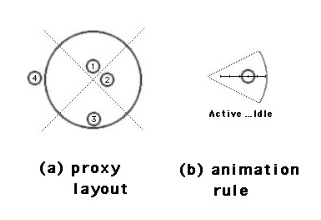
\includegraphics[width=0.5\linewidth]{figures/babble.png}
        \caption{The illustration on the left shows the layout of the proxy in Babble \cite{ericksonSocialTranslucenceApproach2000}, where dots 1, 2, and 3 are part of the conversation, and 4 is in another. The illustration on the right shows how the dots animate and drift further away depending on their activity level.}
        \label{fig:babble}
    \end{figure}

    \subsection{Workspace Awareness} \label{sec:sota_awareness}
    
    Endsley \cite{endsleyTheorySituationAwareness1995} defines \textit{awareness} as "\textit{knowing what is going on.}" Several traits have emerged in previous studies on awareness \cite{adamsSituationAwarenessCognitive1995, normanThingsThatMake1993, endsleyTheorySituationAwareness1995, gutwinDescriptiveFrameworkWorkspace2002}: Awareness is the knowledge about the state of the environment in both space and time. Since environments change over time, maintaining and updating this knowledge is part of awareness. Individuals can achieve this by interacting with and exploring the environment. Finally, awareness is not the primary goal of a task-oriented system but rather a secondary goal, the primary objective being to complete the task.

    Situation Awareness (SA) is a concept that arose in research about more dynamic and complex environments with high information load, variable workload, and risk \cite{gabaSituationAwarenessAnesthesiology1995}. Adams et al. \cite{adamsSituationAwarenessCognitive1995} define SA as "\textit{the up-to-the-minute cognizance required to operate or maintain a system.}" Endsley \cite{endsleyTheorySituationAwareness1995} describes a three-stage definition of SA that focuses more on the process. The first stage is the perception of relevant elements in the environment. The second stage is the comprehension of the current situation, or the ability to relate perceptual information retrieved in the first stage with past knowledge to understand their meaning. The third and last stage is the forecast of the status of those elements, which is invaluable for decision-making.
    
    Gutwin and Greenberg \cite{gutwinDescriptiveFrameworkWorkspace2002} define the concept of workspace awareness as "\textit{the up-to-the-moment understanding of another person's interaction with the shared workspace.}" It is a specialized kind of SA due to the shared workspace context -- it is about being aware not only of the environment but also of other individuals and their interactions with that environment. Similarly to Erickson and Kellog \cite{ericksonSocialTranslucenceApproach2000}, they believe the difficulty of maintaining awareness in collaborative tasks in digital systems lies in the technological constraints of the medium, the lack of information due to the limited perception of others, and the misrepresentation of that information.

    To aid the understanding of concepts and purposes of designing workspace awareness in groupware systems, Gutwin and Greenberg \cite{gutwinDescriptiveFrameworkWorkspace2002} developed a three-part conceptual framework. The first part focuses on what information is used and what is necessary for workspace awareness. The second part is about how that information is gathered. Lastly, the third part concerns the application of workspace awareness in collaboration.

    Previous research \cite{dourishAwarenessCoordinationShared1992, sohlenkampIntegratingCommunicationCooperation1994, mcdanielAwarenessCollaborativeSystems1997, gutwinDescriptiveFrameworkWorkspace2002} explore a set of workspace information that people keep track of during collaborative work, which is the elements that answer the questions "\textit{who, what, where, when, and how.}" Gutwin and Greenberg \cite{gutwinDescriptiveFrameworkWorkspace2002} present specific elements and questions answered by those elements according to what they believe is the core of workspace awareness, seen summarized on tables \ref{tab:workspaceElementsPresent} and \ref{tab:workspaceElementsPast}.

   \begin{table}[!ht]
        \centering
        \caption{Elements of workspace awareness of the present \cite{gutwinDescriptiveFrameworkWorkspace2002}.}
        \begin{tabular}{lll}
             \hline
             Category & Element & Questions \\
             \hline
             Who & Presence  & Is anyone in the workspace? \\
             & Identity  & Who is participating? Who is that? \\
             \vspace{0.7em}
            
             & Authorship & Who is doing that? \\
             What & Action & What are they doing? \\
             & Intention & What goal is that action part of? \\
             \vspace{0.7em}
            
             & Artifact & What object are they working on? \\
             Where & Location & Where are they working? \\
             & Gaze & Where are they looking? \\
             & View & Where can they see? \\
             & Reach & Where can they reach? \\
        \end{tabular}
        \vspace{1em}
        
        \label{tab:workspaceElementsPresent}

        \bigskip
        \caption{Elements of workspace awareness of the past \cite{gutwinDescriptiveFrameworkWorkspace2002}.}
        \begin{tabular}{lll}
             \hline
             Category & Element & Questions \\
             \hline
             How & Action history & How did that operation happen? \\
             \vspace{0.7em}
              & Artifact history & How did this artifact come to be in this state? \\
            \vspace{0.7em}
             When & Event history & When did that event happen? \\
             \vspace{0.7em}
             Who & Presence history & Who was here, and when? \\
             \vspace{0.7em}
             Where & Location history & Where has a person been? \\
             \vspace{0.7em}
             What & Action history  & What has a person been doing? \\
            
        \end{tabular}
        \vspace{1em}
        \label{tab:workspaceElementsPast}
    \end{table}


    Earlier findings \cite{segalEffectsChecklistInterface1994, normanThingsThatMake1993, dixHumanComputerInteraction2003, hutchinsTechnologyTeamNavigation1990, gutwinDescriptiveFrameworkWorkspace2002} propose three primary sources and mechanisms for gathering workspace information: through people's bodies and consequential communication, through workspace artifacts and feedthrough, and through conversation, gestures, and intentional communication. People's bodies provide extensive details about their current work, making watching and hearing other people a mechanism for obtaining workspace information \cite{gutwinDescriptiveFrameworkWorkspace2002, segalEffectsChecklistInterface1994}. This mechanism for gathering information is called \textit{consequential communication} \cite{segalEffectsChecklistInterface1994}.

    The second source of information is the artifacts produced in the workspace \cite{dixHumanComputerInteraction2003, gaverSoundSupportCollaboration1991}. The information that can be collected from these artifacts can be obtained either through visible characteristics \cite{gutwinDescriptiveFrameworkWorkspace2002} or through the sound that is made when manipulating them \cite{gaverSoundSupportCollaboration1991}. The mechanism used for gathering this information is called \textit{feedthrough} \cite{dixHumanComputerInteraction2003}, meaning that when manipulating an artifact, information is received by not only the person doing the action as a form of feedback but also by others who are watching.

    The third source of workspace information is conversation and gesture through intentional communication \cite{clarkUsingLanguage1996, heathUnpackingCollaborationInteractional1994, birdwhistellIntroductionKinesicsAnnotation1952}. People can gather information from verbal communication in different ways: through explicit conversational exchange of awareness elements \cite{gutwinDescriptiveFrameworkWorkspace2002}, by picking up relevant information from other peoples' conversations \cite{gutwinDescriptiveFrameworkWorkspace2002}, or through \textit{verbal shadowing} or "outlouds" \cite{heathUnpackingCollaborationInteractional1994} which are comments made by individuals while working that are addressed to no one in particular.

    Gutwin and Greenberg \cite{gutwinDescriptiveFrameworkWorkspace2002} suggest five types of activities that benefit from workspace awareness. The identified types include: the management of coupling -- the degree to which people are working together \cite{salvadorDenverModelGroupware1996} or the amount of work a person can do before requiring the help of another \cite{gutwinDescriptiveFrameworkWorkspace2002}; simplification of communication -- allowing using deictic references, demonstrations, and visual evidence; coordination of actions; anticipation; and assistance.

    % compare workspace awareness and awareness

    \subsection{Spatial Group Interaction in VR} \label{sec:sota_spatial}

    Unlike conventional CSCW settings, real-time collaboration in virtual environments introduces novel interaction possibilities, particularly when multiple users simultaneously engage with one or more objects \cite{brollInteractingDistributedCollaborative1995}. Therefore, it becomes essential to acknowledge the importance of enhancing awareness in this specific context.

    A spatial approach to collaborative virtual environments consists of spaces or rooms allowing individuals to navigate and engage with one another and the objects, or artifacts, within these designated areas \cite{benfordSpatialModelInteraction1993}. With the goal of enhancing collaboration and scalability within large virtual environments, Benford and Falhén \cite{benfordSpatialModelInteraction1993} propose the spatial model of interaction. 

    The spatial interaction model introduces the concepts of medium, aura, awareness, focus, nimbus, and adapters. The medium is the means through which interactions with objects occur, for example, through text, audio, or visuals. The aura represents an area in which objects can interact within a given medium. When two auras collide, the interaction between the objects in the medium becomes possible. Objects can have multiple auras, such as their size, shape, and color.

    Awareness is the basis on which objects control their potential interactions, as determined by their auras. This awareness is not necessarily symmetrical. For example, between object A and object B, object A can be more aware of B than B is aware of A. The awareness of an object towards another is calculated based on the combination of its focus and nimbus. Focus and nimbus are, like auras, subspaces of an object and describe its attention or presence, respectively. Benford and Falhén \cite{benfordSpatialModelInteraction1993} describe this as "the more an object is within your focus, the more aware you are of it and the more an object is within your nimbus, the more aware it is of you".

    Furthermore, Benford and Falhén \cite{benfordSpatialModelInteraction1993} denote that a person does not need to be aware of their aura, focus, and nimbus, as these may be manipulated using natural interactions. Notably, they indicate three main ways of managing these subspaces. The first is through implicit interaction derived from, for example, the movement, orientation, or eye gaze of individuals. The second is through explicit adjustment of parameters, for instance, with the help of a user interface. The third is through adapters which modify a user's aura, focus, and nimbus. An example of an adapter would be a tool that a person can pick up or a table in which a user can sit, altering the user's aura, focus, and nimbus for that context.

    Domingues et al. \cite{dominguesCollaborative3DInteraction2011} develop a workflow-based approach to collaborative 3D interaction based on the spatial model of interactions. They describe the workflow concept, which manages tasks and ensures coordination in collaborative environments. The workflow comprises two components: the shared component, encompassing the data and state information of all users and sources within the environment; and the motor component, which uses the data from the shared component to execute actions on particular sources through assistance functions. Here, a \textit{source} is an object that users can perceive, \textit{particular sources} are objects that change during 3D interaction through assistance functions, serving as support tools, and \textit{assistance functions} help manage coordination in 3D interaction.

    \begin{figure}[h]
        \centering
        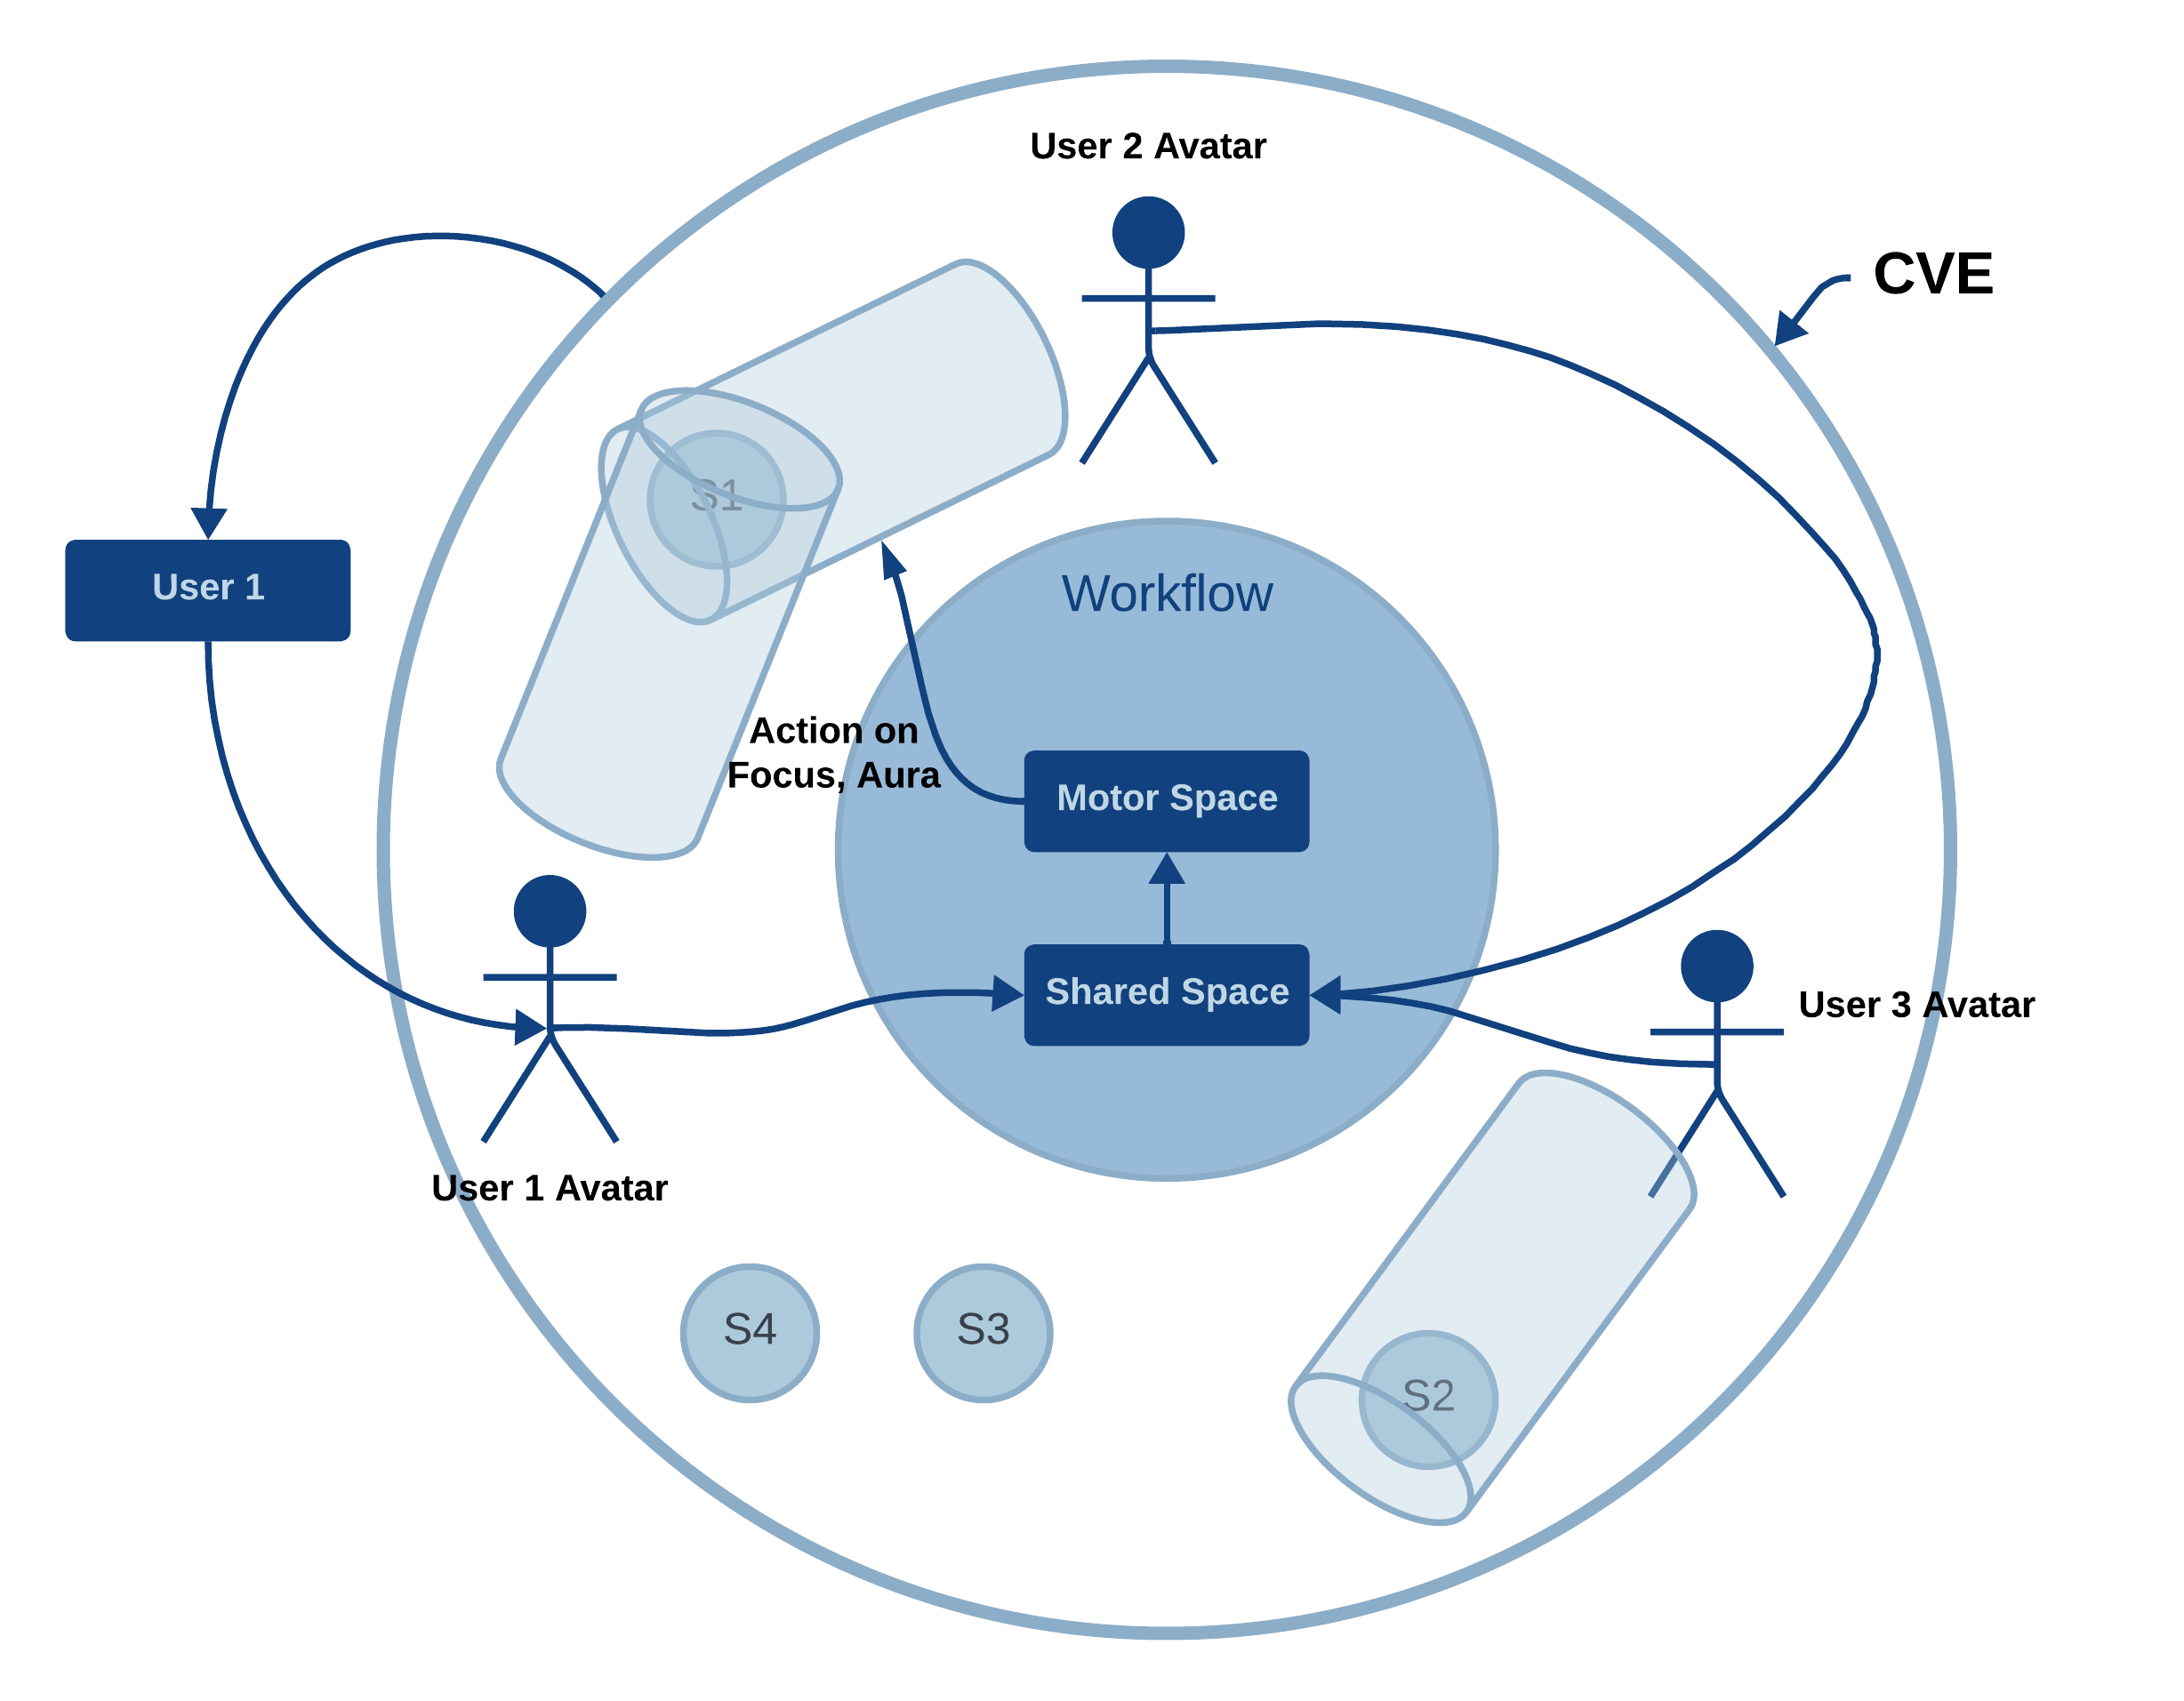
\includegraphics[width=0.9\textwidth]{figures/spatial_model.png}
        \caption{Portrayal adapted from the work of Domingues et al. \cite{dominguesCollaborative3DInteraction2011}. This represents their workflow approach applied to a CVE, where cylinders represent user foci. In this example, the nimbus of the object S1 is the set of users 1 and 2. }
        \label{fig:spatial_model}
    \end{figure}

    Next, they specify five particular sources, dedicated to interaction in the virtual environment. \textit{3DIFocus} coincides with objects the user can interact with, meaning in their field of view. \textit{3DINimbus} symbolizes all users that might interact with this source. \textit{3DIAura} is a zone that enables specific interactions if users are situated within its area. \textit{3DIAssistant} assists users during specific actions through a virtual guide. Lastly, \textit{3DIAvatar} is the digital counterpart of a user. These concepts are illustrated in figure \ref{fig:spatial_model}

    Using this model, Domingues et al. \cite{dominguesCollaborative3DInteraction2011} describe several assistance functions, in particular, an assistance function for helping the coordination of multi-user interaction with an object. They model multi-user interaction by inserting joints between the user avatars and the object, allowing for manipulation of that object using single-user interaction techniques. The assistance function then helps manage this interaction by creating visual guides for the users by changing the color of the avatars engaged in multi-user interaction, or by displaying the object's direction, for instance.
    
%\section{Object Interaction Techniques} \label{sec:sota_interaction}
\begin{comment}
    Bowman and Hodges \cite{bowmanFormalizingDesignEvaluation1999} present a taxonomy of object interaction techniques, categorizing them into three main groups: selection -- choosing an object; release -- releasing an object; and manipulation -- setting the position, orientation, or other characteristics of the selected object. Object manipulations are accomplished by mapping user input, either through physics simulation or programmed behavior  \cite{mendesSurvey3DVirtual2019}. This section primarily details techniques within the manipulation group that involve programmed behaviors, with a few also encompassing selection features.

    Mendes et al. \cite{mendesSurvey3DVirtual2019} extend the taxonomy to differentiate various mapping mechanisms employed in object manipulation techniques. In terms of transformation separation, these mechanisms can be categorized as follows: no transformation separation -- when interactions do not separate degrees of freedom (DoF), \textit{partial} -- when some interactions group DoFs while separating others, and \textit{total} -- when all transformations are applied separately. A study by Mendes et al. \cite{mendesBenefitsDOFSeparation2016a} analyzed the advantages of DoF separation in mid-air 3D object manipulation. The findings indicated that this separation reduced errors while increasing the time required for complex tasks, rendering it more suitable for tasks demanding precision. This conclusion can be extended to other manipulation mediums, such as tabletop interactions.

    Regarding transformation mapping, Mendes et al. \cite{mendesSurvey3DVirtual2019} distinguish between the following approaches: \textit{exact} -- mapping user input directly to the virtual object, \textit{scaled} -- a linear or nonlinear mapping to either increase accuracy with closer objects or increase the range of movement with farther objects, \textit{remapping} -- mapping DoFs onto different DoFs, and \textit{hybrid} -- using a combination of other mapping types for different DoFs.

    Numerous previous studies have investigated the effectiveness of touch-based interactions in the context of DeskVR, exploring various scenarios such as menu navigation \cite{zielaskoMenusDeskSystem2019}, medical image data examination for radiologists \cite{sousaVRRRRoomVirtualReality2017}, travel techniques \cite{amaroDesignEvaluationTravel2022}, and object interaction \cite{almeidaSIT6IndirectTouchbased2023}. The consensus from these studies suggests that, although a touch-based approach may not always be the most time-efficient, it significantly reduces physical strain, enhancing overall comfort and prolonged usage time for individuals. This aspect is essential for DeskVR, where the primary objective is to alleviate physical strain, improve accessibility, and boost productivity \cite{zielaskoRemainSeatedFullyimmersive2017, zielaskoSitNotSit2021}. For this reason, touch-based approaches will be preferred over mid-air interactions.

    It is important to note that touch-based approaches are commonly classified as direct and indirect touch manipulation \cite{mendesSurvey3DVirtual2019}. Direct touch involves users manipulating an object by touching it through a screen display. However, this is impractical in HMD VR, where users cannot see the touch display. Therefore, the most suitable approach is indirect touch manipulation, where users utilize an external touch surface without the need to touch the object directly.
    
    This section is divided into two parts: first, an overview of techniques for single-user object interaction, and second, a discussion of techniques designed for manipulating objects in a multi-user context.

    \subsection{Single User}

    There is a recurring theme in collaborative VR research \cite{pinhoCooperativeObjectManipulation2002, pinhoCooperativeObjectManipulation2008, mortensenCollaborationTeleImmersiveEnvironments2002, otmaneCollaborative3DInteraction2007} that emphasizes a preference for employing single-user techniques in collaboration rather than designing specific multi-user approaches. The rationale behind this choice is to allow users to utilize techniques that are more familiar and easier for them to understand, as these approaches are extensively researched and widely known. As such, an examination of single-user interaction is relevant.

    % mid-air

    \cite{bowmanEvaluationTechniquesGrabbing1997, wilkesAdvantagesVelocitybasedScaling2008}
    \cite{mendesBenefitsDOFSeparation2016a}

    % touch
    
    \cite{martinetEffectDOFSeparation2010}
    \cite{sousaVRRRRoomVirtualReality2017}
    \cite{simeoneIndirectTouchManipulation2016}
    \cite{almeidaSIT6IndirectTouchbased2023}

    \subsection{Multi-User}

    \cite{riegeBentPickRay2006}
    \cite{duvalSkeweR3DInteraction2006}
    \cite{chenechalWhenGiantMeets2016}
    \cite{grandiDesignEvaluationHandheldbased2017}
\end{comment}

\section{Concurrency Control} \label{sec:sota_concurrency}

    Margery et al. \cite{margeryGeneralFrameworkCooperative1999} developed a classification to assess the cooperation levels in multi-user systems. In systems with level 1 collaboration, users can perceive and communicate with each other in the virtual world through avatars. Level 2 systems enable users to manipulate objects within the scene. Level 3 systems allow users to manipulate the same object simultaneously. Level 3 can be further subdivided based on the degree of independence in users' actions, such as independently changing different aspects of an object or combining inputs codependently. This last collaborative level, particularly the codependent mode, is considered the most natural and immersive form of collaboration, offering enhanced efficiency.
    
    Broll \cite{brollInteractingDistributedCollaborative1995} had previously defined something similar to levels 2 and 3, cooperative and collaborative interaction, respectively. Recognizing which interactions are concurrent and which are not is essential yet challenging. Without a notion of simultaneity, interactions become a series of individual moves by each user rather than a coordinated combination. In distributed environments, typical in collaborative virtual reality, where each user has a copy of the world, determining concurrency is complicated, especially considering communication delays.
 
    Concurrency control prevents conflicts of concurrent updates arising from adverse network conditions. In its absence, users manipulating shared objects in conflicting directions may experience difficulty anticipating outcomes and encounter divergence of state \cite{robertsControllingConsistencyCollaborative2004}, introducing confusion among participants, offering disparate views of what should be a shared world and, in turn, violating the essential consistency requirement \cite{sungConcurrencyControlCIAO1999}. Therefore, the study of concurrency control emerges as an essential research topic for developing systems with level 3 collaboration.

    The following subsections describe three distinct approaches for implementing concurrency control. Object ownership methods use locking mechanisms to block users from interacting with an object or its properties unless they possess a corresponding lock or ownership. Attribute separation methods assign specific attributes or degrees of freedom of an object to individual users, making each user responsible for that attribute. Finally, distributed average techniques calculate the average of participants' actions, integrating and updating them distributively.

    \subsection{Object Ownership Techniques}

    Greenberg and Marwood \cite{greenbergRealTimeGroupware1994} describe how traditional concurrency control strategies can be used in real-time groupware systems. In particular, they demonstrate how the method of privileged access through locking can be applied in these systems, describing two different approaches. A non-optimistic locking policy blocks users from interacting with an object until a lock has been granted, signifying ownership over the object. An optimistic locking policy allows users to manipulate an object before they know if a lock has been granted to them. If the lock has been denied, the object returns to its original state, and a repair must be done. Optimistic locking schemes can be further divided into two approaches. A fully-optimistic approach allows users to manipulate multiple objects with tentative locks, while a semi-optimistic approach only allows users to manipulate one object at a time.

    BrickNet \cite{singhBrickNetSoftwareToolkit1994a} is a toolkit for network-based virtual environments. It uses a pessimistic locking mechanism for object manipulation where objects can only be updated by the current owner. Users have to request ownership over an object to the server, and the server mediates object updates. DIVE \cite{hagsandInteractiveMultiuserVEs1996} is a multi-user distributed virtual environment system. DIVE also employs a pessimistic locking mechanism, similar to BrickNet, where users require an object-based token to interact with the object. Spline \cite{watersDiamondParkSpline1997} is a software platform for developing distributed virtual environments that implements the Interactive Sharing Transfer Protocol, or ISTP \cite{watersDesignInteractiveSharing1997}. Objects in the ISTP protocol, like DIVE, are only subject to changes from its owner process. This ownership can be transferred between processes. CAVERNsoft \cite{leighCAVERNDistributedArchitecture1997} is a collaborative software architecture that was used by the CAVE Research Network, which also uses the pessimistic locking approach.

    The PaRADE collaborative environment \cite{robertsMaximisingConcurrencyScalability1997, robertsControllingConsistencyCollaborative2004} takes a different approach to pessimistic locking by employing a predictive strategy. Developed to mitigate adverse network effects, PaRADE aims to enhance both responsiveness and consistency through advanced time management. In PaRADE, all events are timestamped with both wall-clock time and causal time, and efforts are made to predict events to reduce the impact of network delays. Combining these times is used for sufficient causal ordering, serving as a middle ground for Lamport's causal ordering \cite{lamportTimeClocksOrdering1978} to enhance concurrency and responsiveness. This approach restricts changes to an object to originate from a single user, leading to the adoption of a predictive object transfer paradigm that anticipates entity ownership in advance.

    The predictive object ownership transfer relies on application knowledge and heuristics to anticipate a user's intention to interact with an object, enabling the transfer in advance of the ownership to minimize the impact of network delays. This advance transfer is important for optimizing responsiveness and in scenarios where ownership may have been erroneously transferred, allowing for retransmission to the correct recipient. Yang and Lee \cite{yangScalablePredictionBased2000} identified scalability challenges in the widespread dissemination of token requests to all users in the network. In response, they introduced the concept of an entity radius, wherein messages are selectively delivered only to individuals within this radius, forming an "entity-centric multicast group."
    
    Pessimistic approaches for locking mechanisms help preserve data integrity in databases, for example. However, in settings such as collaborative virtual environments (CVEs), not only does obtaining a lock necessitate user waiting, but ensuring sequential updates becomes less scalable with a growing number of users. Sung et al. introduce CIAO \cite{sungConcurrencyControlCIAO1999}, a large-scale 3D layout system that uses a semi-optimistic policy for managing shared object manipulation to enhance responsiveness. Unlike traditional systems, users in CIAO can manipulate objects without waiting for a lock. To address potential confusion arising from multiple users interacting with an object, the CIAO interface incorporates awareness features, using translucent clones to indicate ongoing manipulations yet to be validated. The authors also address the challenges of concurrently interacting with hierarchically related objects.
    
    \subsection{Attribute Separation Techniques} \label{sec:dof_concurrency}

    The approaches discussed in the previous section are limited to a collaboration level of 2, as there is no stage where multiple users synchronize their inputs on a shared object. Additionally, those concurrency control mechanisms often introduce issues commonly called "surprise" \cite{linebargerConcurrencyControlMechanisms2004}. Such surprises manifest as conflicts leading to the reversal of changes or unexpected alterations in the anticipated order of events due to concurrency control conflicts. 
    
    This section introduces strategies that elevate collaboration to level 3, enabling independent modifications of various attributes of an object simultaneously. The concept involves assigning ownership of specific attributes to individual users, allowing multiple users to collaboratively manipulate an object without needing sequential ownership.
    
    In their work, Lee et al. \cite{leeSupportingFineGrainedConcurrent2012} refer to the manipulation of an attribute of a shared object as a "task." However, they explain the importance of avoiding "surprises" or, in this context, "task-surprises." These surprises may arise when interruptions occur during user tasks by other tasks or when task dependencies result in unexpected states when executed concurrently.

    \begin{figure}[h!]
        \centering
        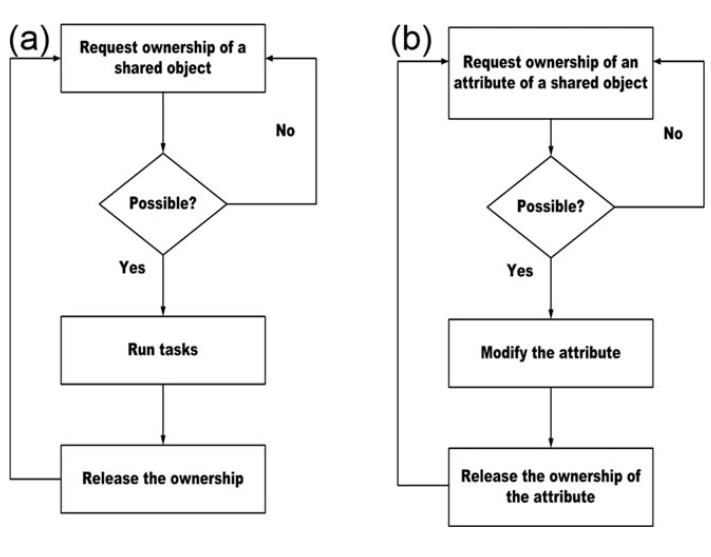
\includegraphics[width=0.65\linewidth]{owner_vs_attr_2.png}
        \caption{Illustration depicting the difference between ownership transfer and attribute separation \cite{leeSupportingFineGrainedConcurrent2012}.}
        \label{fig:enter-label}
    \end{figure}

    % TODO: I am mixing here distributed and dof techniques, can't really think of a nice way of doing this introductory part
    Advancements in internet infrastructure around the turn of the century, particularly with the establishment of Internet2 \cite{yeungInternetScalingBackbone1997} -- a robust network implemented in the United States in 1996 for academic purposes -- sparked new interest in exploring collaborative tasks in remote environments. Mortensen et al. \cite{mortensenCollaborationTeleImmersiveEnvironments2002} aimed to assess the feasibility of joint tasks when two users, separated by thousands of miles, interacted in a shared virtual environment within DIVE. The specific task involved both users lifting a stretcher together and moving it along a predefined path into a building. To achieve this, two handles were added to the stretcher for the users to manipulate, with the stretcher aligning itself based on the position and orientation of these handles. Their findings revealed that while data transmission speeds and throughput were sufficient, the lack of software support, particularly concerning lost data packets impacting consistency, posed a significant challenge.

    Roberts et al. \cite{robertsConstructingGazeboSupporting2003} investigated two distinct methods of shared object manipulation and how these methods were influenced by the display devices their users employed: an immersive walk-in display with tracked head and hands, and a desktop application. The two methods explored were sharing the same attribute and sharing through different attributes. To conduct this study, they devised an experiment where users collaborated on constructing a gazebo in DIVE. Some sub-tasks required users to collaborate using the same attribute, such as jointly carrying a beam, while other tasks involved simultaneous manipulation of the object for different purposes, such as one person inserting a screw while another held the beam in place. This study also concluded that technological advancements had made such collaborative tasks feasible, but the ownership mechanism of DIVE failed to provide effective collaboration \cite{robertsSupportingCloselyCoupled2005a}. As such, it became evident that new systems needed to be developed with level 3 collaboration in mind.

    Pinho et al. \cite{pinhoCooperativeObjectManipulation2002, pinhoCooperativeObjectManipulation2008} proposed a method for collaborative object interaction by separating degrees of freedom (DoF) and assigning them to different users. A degree of freedom in this context refers to a degree of control over the movement of an object, such as horizontal translation or rotation around an axis. As previously mentioned in section \ref{sec:sota_interaction}, the separation of DoF can be beneficial when precision is an important factor.
    
    The goal of this approach was to use single-user interaction techniques, such as HOMER \cite{bowmanEvaluationTechniquesGrabbing1997, mossel3DTouchHOMERSIntuitive2013}, in collaborative manipulation, with the reasoning that they were well-researched, commonly understood, and perceived as more "magical" than natural, which was prevalent in most collaborative manipulation techniques then. The objective was to extend users' capabilities for multi-user object interaction. Additionally, the authors focused on awareness by implementing features like using a pointer to indicate the selected object, changing the object's color based on its state, and representing the DoF graphically, as shown in Figure \ref{fig:pointer}. While the results were positive, two challenges were identified: testing the applicability with more than two users, and the selection of DoF for each user was predetermined in a configuration, limiting flexibility.

    \begin{figure}[h!]
        \centering
        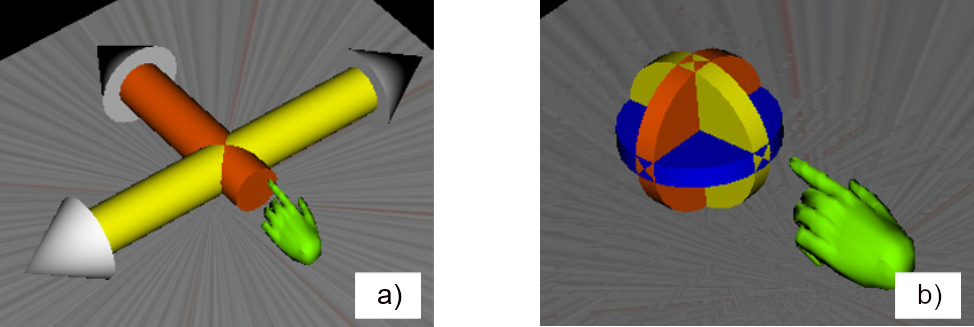
\includegraphics[width=.96\textwidth]{figures/pointer.png}
        \captionof{figure}{Illustration of translation (a) and rotation (b) pointers in \cite{pinhoCooperativeObjectManipulation2008}}
        \label{fig:pointer}
    \end{figure}
    

    Lee et al. \cite{leeSupportingFineGrainedConcurrent2012} proposed a concurrency control mechanism based on fine-grained tasks. In this approach, if a user who does not own an object requests a task to manipulate a shared object, the task is permitted if it avoids conflicts with the owner's task and does not lead to task surprises. If the task is not allowed, non-owners can perform their tasks with duplicates of the object on a personal workspace, similar to the ghost images in CIAO \cite{sungConcurrencyControlCIAO1999}. The outcomes of these modifications in personal workspaces can be stored, allowing users to discuss and determine the final state of the object. Figure \ref{fig:sota_finegrained} demonstrates the flow of the concurrency control process. 

    \begin{figure}[ht!]
        \centering
        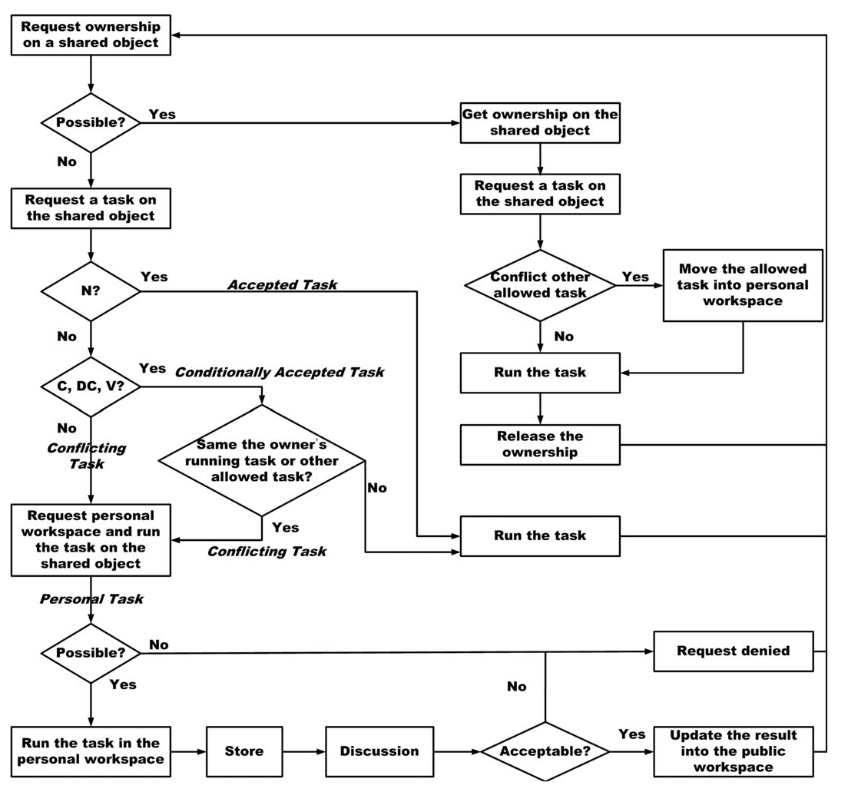
\includegraphics[width=1\linewidth]{figures/finegrainedtasks.png}
        \caption{Illustration of the fine-grained task concurrency control system by Lee et al. \cite{leeSupportingFineGrainedConcurrent2012}.}
        \label{fig:sota_finegrained}
    \end{figure}

     The allowance types for each task classification can be seen on Table \ref{tab:sota_finegrained}. \textit{Conflicting tasks} are exclusive to the object's owner. \textit{Conditionally accepted tasks} can be executed only if no one else is performing the task, while \textit{accepted tasks} can always be executed. While their implementation demonstrated slower efficiency compared to other attribute-sharing mechanisms, Lee et al.'s approach reduced the occurrence of task surprises.

    \begin{table}[h!]
        \centering
       \caption{Allowance type for each task classification by Lee et al. \cite{leeSupportingFineGrainedConcurrent2012}.}
        \begin{tabular}{m{12em} l}
            \hline
            Classification of Tasks & Allowance Type  \\
            \hline
            Translation & Conflicting task \\
            Rotation & Conflicting task \\
            Scaling & Conflicting task \\
            Fission & Conflicting task \\
            Merge & Conflicting task \\
            New & Accepted task \\
            Remove & Conflicting task \\
            Copy & Conditionally accepted task \\
            Data calculation & Conditionally accepted task \\
            Visual property & Conditionally accepted task \\
        \end{tabular}
 
        \label{tab:sota_finegrained}
    \end{table}
    
    \subsection{Distributed Average Techniques} \label{sec:average_concurrency}

    This section explores techniques associated with codependent level 3 collaboration. Integrating level 3 collaboration into CVEs is challenging, especially in regards to the complexity of combining and integrating actions from multiple users, the absence of feedback inherent in physical interactions with an object, and network communication issues, especially concerning latency, which significantly influences the ability to detect simultaneous actions \cite{ruddleSymmetricAsymmetricAction2002, brollInteractingDistributedCollaborative1995}.
    
    Ruddle et al. \cite{ruddleSymmetricAsymmetricAction2002} investigated whether an asymmetric or symmetric approach was better suited for level 3 collaboration in the piano mover's task. This task involves two users maneuvering a large virtual object through confined spaces. Symmetric manipulation requires coordinated actions in direction and intensity, while asymmetric manipulation allows users to interact with the object differently, considering the average of the interactions. To address latency concerns, experiments were conducted on a single host computer. Interestingly, the results did not reveal a significant difference in the time participants took to complete the task, but instead, that performance depended on the task. However, the study highlighted the challenge of coordinating participants' movements, emphasizing the need for feedback, whether haptic or otherwise.

    Friston et al. \cite{fristonConsensusBasedNetworking2022} present a concurrency control framework designed to enable the integration of level 3 collaboration in distributed virtual environments. This approach views the collaborative environment as a distributed data-fusion problem and incorporates elements such as prediction, distributed averaging, continuous authority, and constraint duplication. The methodology is rooted in consensus-based networking, where simulations share state updates with other nodes, and local solvers integrate these updates to establish a distributed average consensus of the system's state, ensuring consistency over time. Unlike bilateral operation or force-reflection systems, where clients submit inputs to a central authority, this approach calculates actions distributively, resulting in improved scalability. The authors conducted experiments that demonstrated the effectiveness of this technique in preserving causality, stacking objects, enabling level 3 collaboration, and providing support for haptic feedback.

\section{DeskVR Interaction} \label{sec:sota_interaction}

    Before the widespread adoption of stereoscopic displays, various effective approaches emerged for utilizing a multi-touch tabletop surface to interact with 3D objects with minimal fatigue \cite{benkoBalloonSelectionMultiFinger2007, strothoffTriangleCursorInteractions2011, daiberBalloonSelectionRevisited2012}. Balloon Selection \cite{benkoBalloonSelectionMultiFinger2007} employs the metaphor of manipulating a balloon attached to a string. This approach divides a 3DOF positioning task into a 2DOF positioning task with one finger on the touch surface and a 1DOF string-pulling task with the other finger to control the height of the balloon. Pulling the fingers apart decreases the balloon's height and bringing them together increases its height. Balloon selection does not differentiate between right and left hands; instead, it prioritizes the order in which fingers are placed on the surface, designating the primary finger (anchor), secondary finger (stretching finger), and tertiary finger (selection finger). This design allows both right-handed and left-handed users to use the technique effortlessly. Additionally, the stretching finger may not always be held, allowing the balloon's height to remain fixed when removed. This feature, referred to as "\textit{String Height Clutching}" by the authors, enables the extension of the balloon's height infinitely. This technique has shown low error rates, likely due to the user's hands being supported by the tabletop surface, resulting in significantly reduced hand tremor and arm fatigue.

    \begin{figure}[ht!]
        \centering
        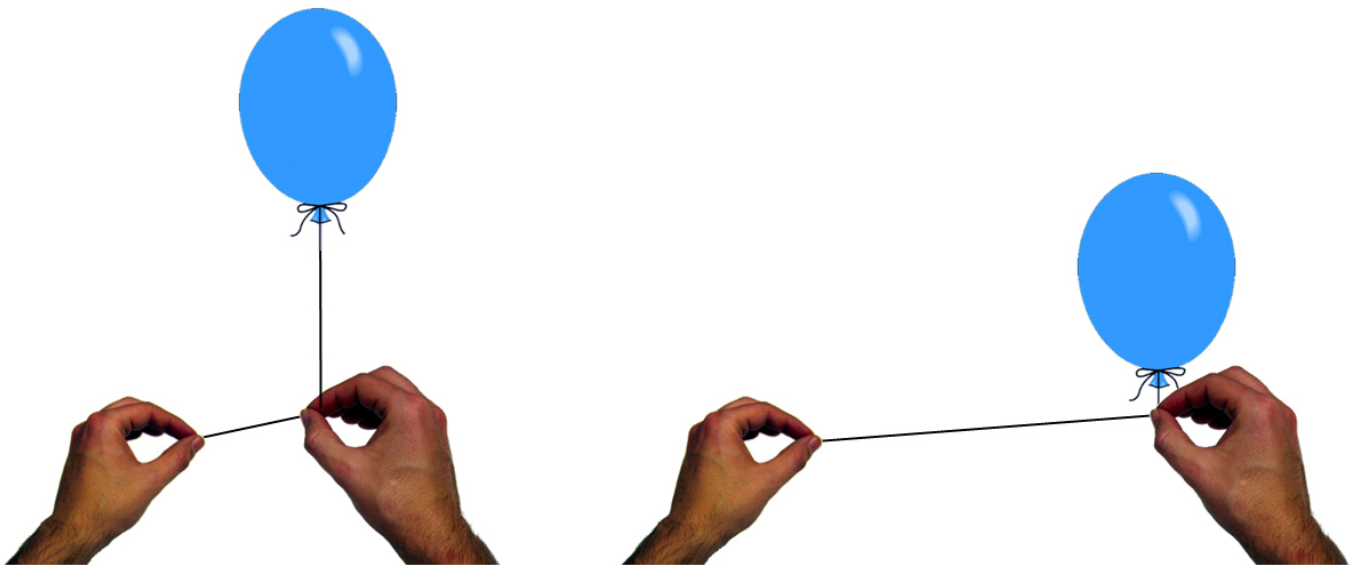
\includegraphics[width=1\linewidth]{figures/balloon_selection.png}
        \caption{Illustration of the Balloon Selection metaphor \cite{benkoBalloonSelectionMultiFinger2007}.}
        \label{fig:sota_balloon}
    \end{figure}

    Corkscrew Selection \cite{daiberBalloonSelectionRevisited2012}, similar to Balloon Selection, also breaks down the 3DOF task into a 2DOF positioning task and a 1DOF height task. However, it differs in the method used to adjust the height of the selection point, achieved through a rotational motion around a selection widget.
    
    Triangle Cursor \cite{strothoffTriangleCursorInteractions2011}, on the other hand, creates an isosceles triangle with its two base vertices positioned at the touch points of two fingers, while the altitude's base point is located at the midpoint. Manipulating the triangle's position involves moving the fingers on the surface, while adjusting its height is controlled by scaling the triangle similarly to a typical pinch gesture based on the distance between the two fingers. The height's upper limit is constrained by the diagonal of the touch surface. Additionally, users can initiate yaw rotation around an axis perpendicular to the table's surface by rotating the fingers around the midpoint.

    In their evaluation comparing Triangle Cursor to Balloon Selection, the authors noted a slight preference in terms of speed and error minimization for Triangle Cursor. However, it's worth mentioning that the tasks necessitated the use of rotational techniques, which required an extension of Balloon Selection by using the rotation of the secondary finger around the primary finger as rotational input.

    \begin{figure}[ht!]
        \centering
        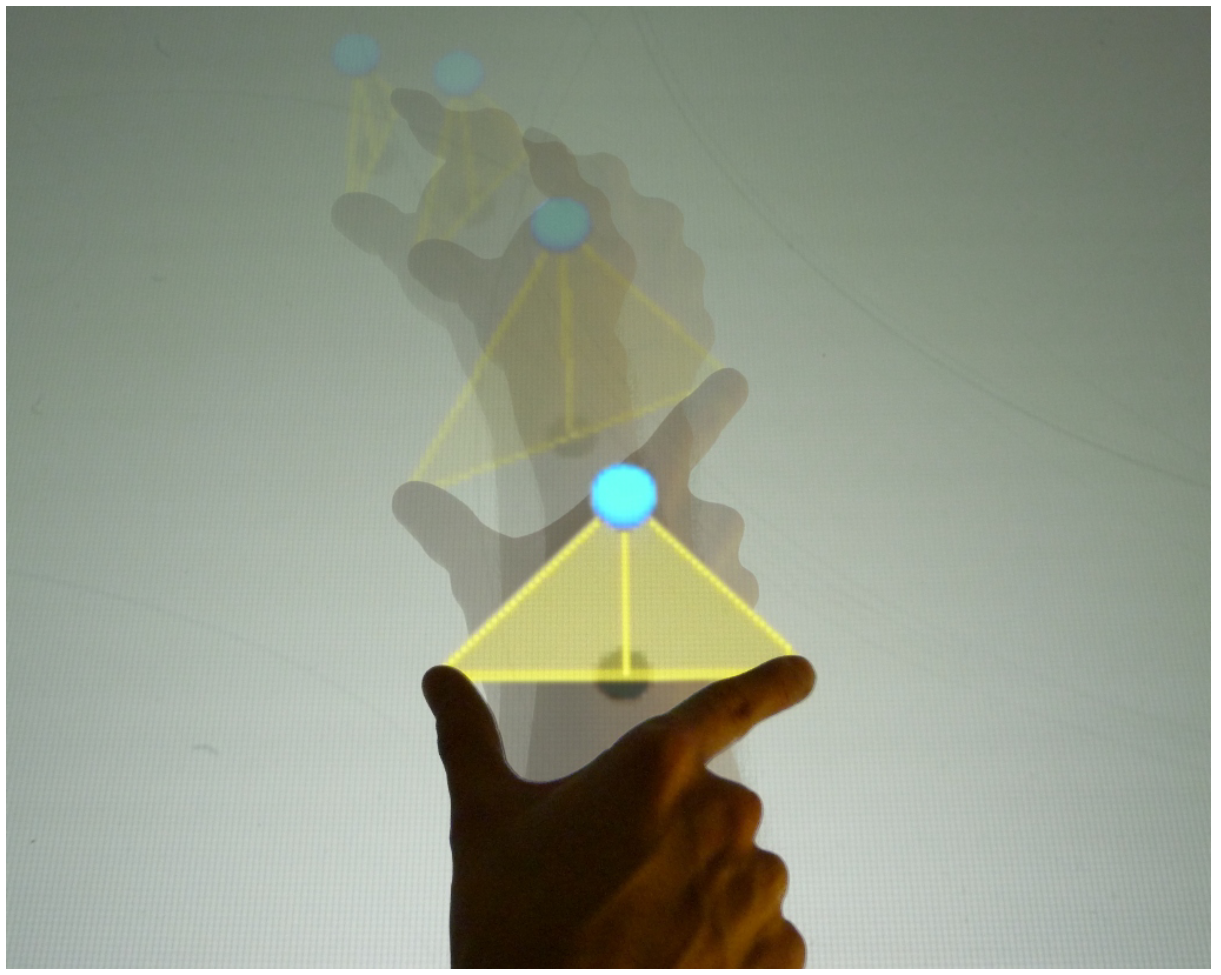
\includegraphics[width=0.6\linewidth]{figures/triangle_cursor.png}
        \caption{Illustration of the Triangle Cursor technique \cite{strothoffTriangleCursorInteractions2011}.}
        \label{fig:sota_triangle}
    \end{figure}


   Zielasko et al. \cite{zielaskoRemainSeatedFullyimmersive2017} introduced the concept of DeskVR, a fully immersive VR experience accessed entirely from an office desk while the user remains seated. Initially conceived to integrate with the workflow of data analysts, the application of this concept extends to broader applications, aiming to alleviate physical strain associated with standing, extend work periods, enhance accessibility, and boost overall productivity.

    Zielasko et al. \cite{zielaskoSitNotSit2021} surveyed to evaluate the advantages and disadvantages of standing versus sitting and the degree of embodiment in virtual reality experiences. The findings indicated that sitting generally scored higher in reducing cybersickness, enhancing comfort, ensuring safety, and improving accessibility. On the other hand, standing was preferred for perceived self-motion, locomotion preciseness, and engagement.

    Given the constraints of DeskVR, environmental interactions must be re-evaluated, especially regarding selection, manipulation, and travel techniques. Because users remain seated in DeskVR, this enables interactions not common in typical VR scenarios, such as touch-based interactions on a desk. Zielasko et al. \cite{zielaskoMenusDeskSystem2019} explored this concept through the evaluation of four menu interaction arrangements in DeskVR: "Desk" aligns menus with the virtual desk, "Air" aligns menus with the user's task, and "DeskPlus" and "AirPlus" combine the previous scenarios with a physical desk to provide passive haptics. These configurations can be seen in Figures \ref{fig:sota_desk_z} and \ref{fig:sota_desk_z2}. The results revealed diverse individual preferences for menu configurations. Some favored desk-aligned menus for tangibility, while others found it odd to touch a menu expected to be virtual. Additionally, menus aligned with the virtual desk required more head movement, making them less efficient. However, variants with a physical desk were favored for reducing physical strain.
    
    \begin{figure}[h!]
        \centering
        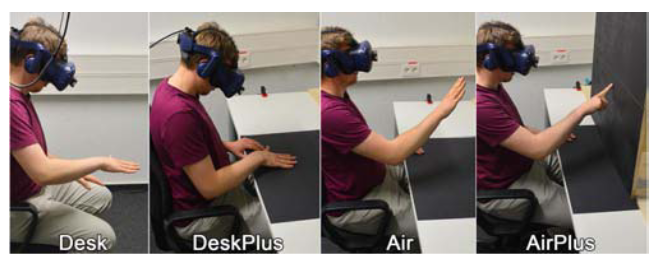
\includegraphics[width=0.85\linewidth]{figures/menu_desk.png}
        \caption{The four different scenarios studied in \cite{zielaskoMenusDeskSystem2019}. The "Desk" scenario aligns the menu with a virtual desk, while the "Air" scenario aligns the menu with the task. The "DeskPlus" scenario aligns the virtual desk with a physical desk, while "AirPlus" aligns the menu with the taks and a vertical board.  }
        \label{fig:sota_desk_z}
    \end{figure}

    \begin{figure}[h!]
        \centering
        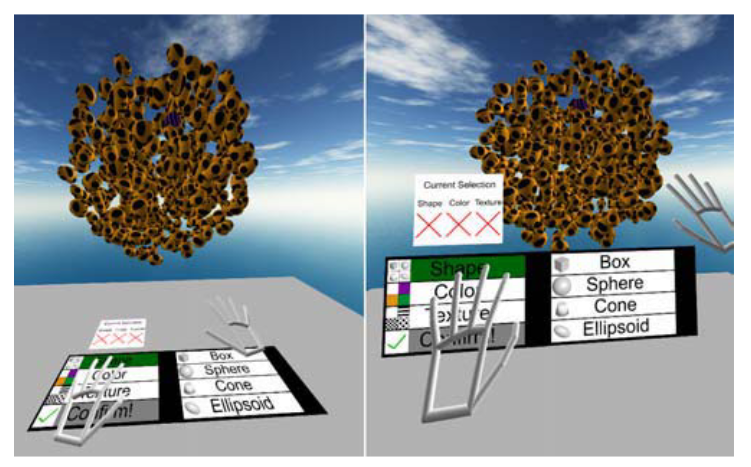
\includegraphics[width=0.85\linewidth]{sota_desk_menu.png}
        \caption{Experimental settings in \cite{zielaskoMenusDeskSystem2019} for desk-aligned menus on the left and task-aligned menus on the right.}
        \label{fig:sota_desk_z2}
    \end{figure}

    Sousa et al. \cite{sousaVRRRRoomVirtualReality2017} introduced VRRRRoom, a VR radiology reading room with a desktop surface for interacting with medical images. Medical images are displayed in 3D above a virtual desk and can be manipulated using indirect touch controls. Users can change volume slices and adjust brightness with their left hand, while rotating the image and changing the scale can be done with their right hand, as depicted in Figure \ref{fig:vroom_gesture}. The gesture-based interaction minimizes the need for users to move their head to view controls, as illustrated in Figure \ref{fig:vroom_desk}.

    \begin{figure}[h!]
        \centering
        \begin{minipage}[t]{.45\textwidth}
          \centering
          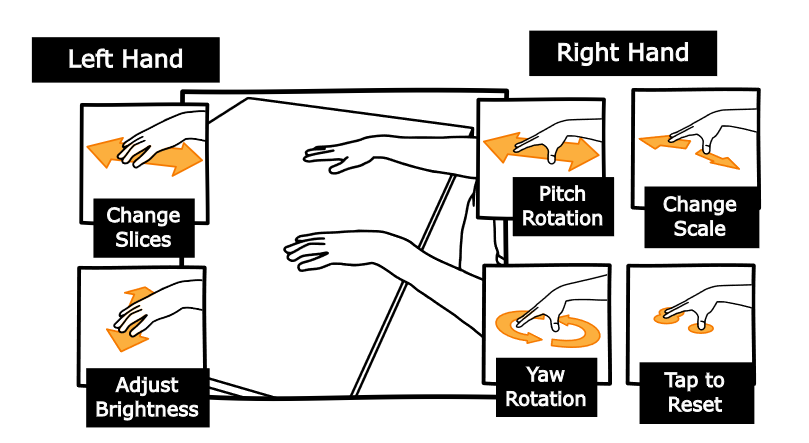
\includegraphics[width=1\textwidth]{figures/vroom_gesture.png}
          \captionof{figure}{Gesture dictionary in \cite{sousaVRRRRoomVirtualReality2017}}
          \label{fig:vroom_gesture}
        \end{minipage}%
        \hspace{0.05\textwidth}
        \begin{minipage}[t]{.45\textwidth}
          \centering
          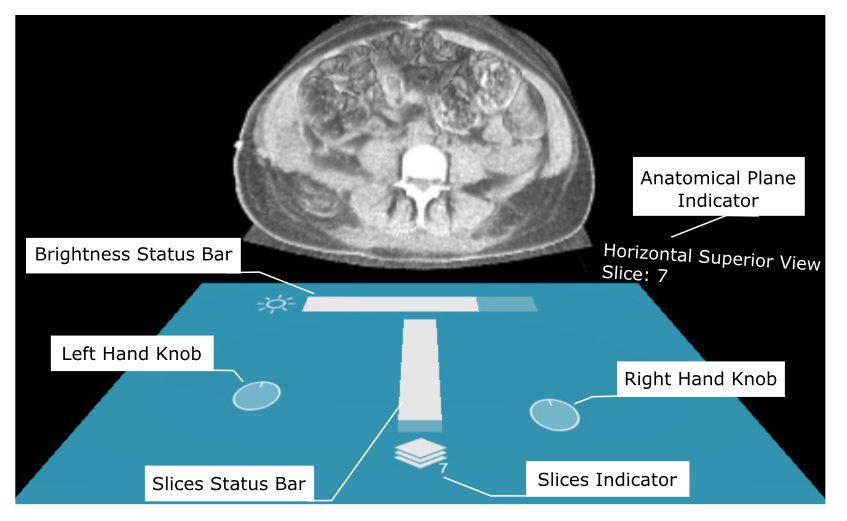
\includegraphics[width=1\textwidth]{figures/vroom_desk.png}
          \captionof{figure}{Virtual desk, control indicators, and medical images rendering in  \cite{sousaVRRRRoomVirtualReality2017}}
          \label{fig:vroom_desk}
        \end{minipage}
    \end{figure}

    The visualization of controls on a virtual desk, exemplified in VRRRRoom \cite{sousaVRRRRoomVirtualReality2017} and illustrated in Figure \ref{fig:vroom_desk}, serves as a valuable tool for instructing users about available gestures and conveying information such as the current volume slice. Zielasko et al. \cite{zielaskoNonStationaryOfficeDesk2019} conducted an experiment to assess the impact of introducing this virtual desk into the virtual environment, analyzing its effects on performance, cybersickness, and presence. Their findings indicated no significant differences in the evaluated aspects, suggesting the potential for expanding the desk functionality to incorporate menus or controls.

    Regarding the selection and manipulation of 3D objects, many techniques are viable in both standing and sitting positions. However, techniques requiring extra controllers may be less suitable, as finding them after being set down while immersed in an HMD can be difficult \cite{zielaskoRemainSeatedFullyimmersive2017}. Almeida et al. \cite{almeidaSIT6IndirectTouchbased2023} developed a DeskVR-specific object manipulation technique called SIT6. This indirect touch-based technique utilizes a gesture dictionary with separated degrees of freedom: three for translation and three for rotation, as seen in Figure \ref{fig:sota_sit6}.  Indirect touch means that users do not directly touch the object through a screen display but interact with it indirectly, as the former would not be practical in VR using an HMD \cite{mendesSurvey3DVirtual2019}. While SIT6 may not be as fast as other state-of-the-art mid-air techniques, it was found to be as effective and less physically demanding.

    \begin{figure}[h]
        \centering
        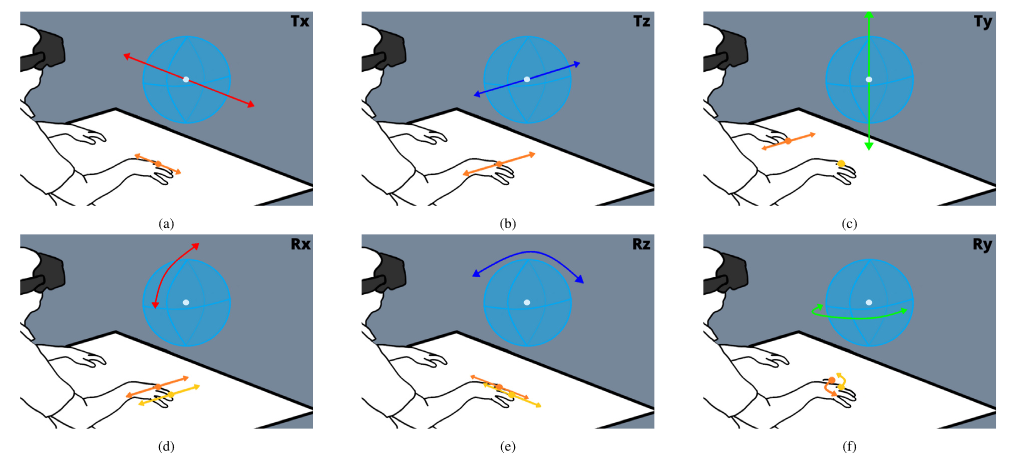
\includegraphics[width=1\linewidth]{figures/sit6.png}
        \caption{The gesture dictionary of SIT6 \cite{almeidaSIT6IndirectTouchbased2023}. Gestures (a), (b), and (c) represent translation movements, while gestures (d), (e), and (f) represent rotation movements.}
        \label{fig:sota_sit6}
    \end{figure}

    Designing traveling techniques in DeskVR is challenging because users are seated, rendering real walking impractical despite its potential presence enhancement. While presence is crucial for reducing cybersickness \cite{zielaskoRemainSeatedFullyimmersive2017}, an effective travel technique in DeskVR should aim to enhance presence without necessitating tiring motions or additional body tracking, such as leg movements. Amaro et al. \cite{amaroDesignEvaluationTravel2022} devised three travel and four orientation techniques, seen in Figure \ref{fig:sota_travel}. One travel technique utilized a VR controller named Continuous Directional Movement. In contrast, the others employed a touch surface and gestures, known as Dog Paddle and Drag'n Go.

    \begin{figure}[h!]
        \centering
        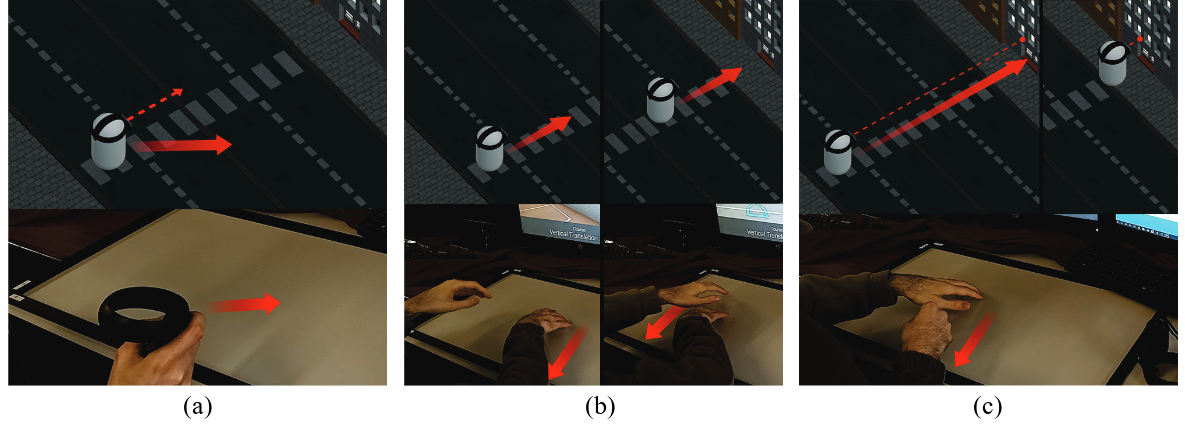
\includegraphics[width=1\textwidth]{figures/sota_travel.png}
        \captionof{figure}{Travel techniques designed for DeskVR by Amaro et al. \cite{amaroDesignEvaluationTravel2022}: Continuous Directional Movement (a), Dog Paddle (b), Drag'n Go (c).}
        \label{fig:sota_travel}
    \end{figure}

    For orientation, Amaro et al. \cite{amaroDesignEvaluationTravel2022} introduced two techniques utilizing VR controllers, named Continuous Directional Rotation and Choose \& Click, one technique utilizing a tactile surface, named Tactile Surface Dragging, and one technique relying on the orientation of the user's head, named Gaze Convergence. These techniques are illustrated in Figure \ref{fig:sota_orientation}. Among the movement techniques, Continuous Directional Movement outperformed its counterparts in performance and comfort, although it appeared to induce more nausea than Dog Paddle. The discomfort in Dog Paddle could stem from its repetitive, exaggerated motions, indicating a potential avenue for exploring more straightforward and less straining interactions. Concerning orientation, Tactile Surface Dragging exhibited superior overall performance, showing fewer cybersickness symptoms than Continuous Directional Rotation, which exhibited the most.

    \begin{figure}[h!]
        \centering
        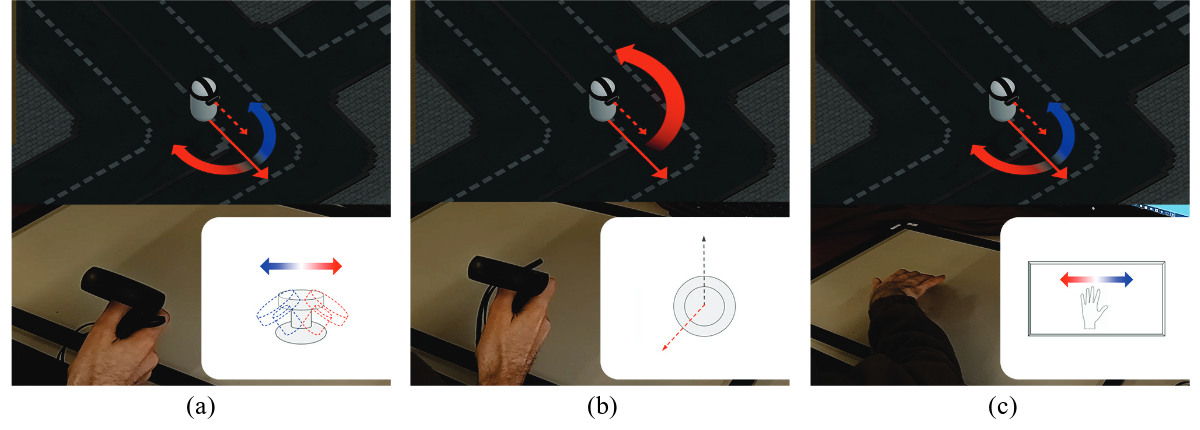
\includegraphics[width=1\textwidth]{figures/sota_orientation.png}
        \captionof{figure}{Orientation techniques designed for DeskVR by Amaro et al. \cite{amaroDesignEvaluationTravel2022}: Continuous Directional Rotation (a), Choose \& Click (b), Tactile Surface Dragging (c).}
        \label{fig:sota_orientation}
    \end{figure}


\section{Discussion} \label{sec:sota_discussion}

    The key takeaway in developing interactions for DeskVR is prioritizing user comfort and leveraging the potential benefits of having a desk in front of the user while being mindful of the associated constraints. Numerous studies have investigated the effectiveness of touch-based interactions in both non-steroscopic contexts, such as Balloon Selection \cite{benkoBalloonSelectionMultiFinger2007}, Corkscrew Selection \cite{daiberBalloonSelectionRevisited2012}, and Triangle Cursor \cite{strothoffTriangleCursorInteractions2011}, and in the context of DeskVR, exploring various scenarios such as menu navigation \cite{zielaskoMenusDeskSystem2019}, medical image data examination for radiologists \cite{sousaVRRRRoomVirtualReality2017}, travel techniques \cite{amaroDesignEvaluationTravel2022}, and object interaction \cite{almeidaSIT6IndirectTouchbased2023}. The consensus from these studies suggests that, although a touch-based approach may not always be the most time-efficient, it significantly reduces physical strain, enhancing overall comfort and prolonged usage time for individuals. This aspect is essential for DeskVR, where the primary objective is to alleviate physical strain, improve accessibility, and boost productivity \cite{zielaskoRemainSeatedFullyimmersive2017, zielaskoSitNotSit2021}. For this reason, touch-based approaches seem preferable over mid-air interactions. Furthermore, Zielasko et al. \cite{zielaskoNonStationaryOfficeDesk2019} demonstrated that presenting a virtual table as a surrogate for the physical table has minimal impact on task performance, cybersickness, and presence, making it a viable option for menus and other interactions without compromising the user experience.
    
    The absence of physical feedback during simultaneous interactions by multiple users creates unpredictability in real-time multi-user collaboration \cite{ruddleLevelsControlCollaborative2003}. While haptic devices like the Phantom Omni \cite{silvaPHANToMOMNIHaptic2009} offer a potential solution by allowing users to manipulate objects and perceive forces applied by others \cite{ruddleSymmetricAsymmetricAction2002}, their integration into DeskVR, potentially involving substitutional reality -- replacing real physical objects such as haptic devices with virtual counterparts \cite{simeoneSubstitutionalRealityUsing2015}, is beyond the scope of this work. Furthermore, the limited mobility of users in DeskVR constrains simultaneous multi-user object interaction, particularly when considering physics-based interaction techniques such as concurrency control using consensus-based networking \cite{fristonConsensusBasedNetworking2022}.

    Considering these factors, level 3 collaboration is unsuitable, and thus, there is no need for distributed average concurrency control techniques. Additionally, degree-of-freedom separation techniques appear restrictive in configuration and interaction while potentially confusing and difficult to use. As such, the fine-grained approach of Lee et al. \cite{leeSupportingFineGrainedConcurrent2012} is appealing, allowing users to discuss different object interactions and arrangements while sharing their perspectives. This approach influenced the idea of using the world-in-miniature \cite{stoakleyVirtualRealityonaWim1995} metaphor for the design of Replico, which plays to the strengths of DeskVR.

    Moreover, providing social visibility, awareness, and accountability in collaborative environments is pivotal in shaping how we communicate \cite{ericksonSocialTranslucenceApproach2000, gutwinDescriptiveFrameworkWorkspace2002}. The chosen approach should provide these elements, enabling users to communicate more effectively. For instance, it should indicate who is interacting with an object, its owner, and who is engaged in the conversation, seamlessly integrating these aspects within the DeskVR environment. Additionally, it should leverage the spatial attribute of VR, incorporating a spatial model of interactions \cite{benfordSpatialModelInteraction1993, dominguesCollaborative3DInteraction2011}. Users within the proximity of an object's aura could trigger interactions, such as audio communication, enabling them to focus on the task at hand with fewer distractions. This aligns with the concept of translucence as discussed by Erickson and Kellogg \cite{ericksonSocialTranslucenceApproach2000}.


    %\cite{odaVirtualReplicasRemote2015}
    %\cite{tianUsingVirtualReplicas2023}
